
\section{Documento de Diseño}

El Documento de Diseño es una herramienta que conduce el desarrollo a lo largo del proyecto y deberá estar dispuesto a sufrir diversos cambios desde la etapa de revisión. Contiene, por escrito, todas las especificaciones necesarias para guiar el proyecto de software. Un documento de diseño tiene que ser una referencia estable, detallando todas las partes del software y cómo van a trabajar.

En metodología ágil será necesario utilizar el product backlog como una verdadera guía para el diseño, este se refinará a lo largo del proyecto, principalmente al finalizar cada sprint.

El Product Backlog o Pila de producto, es un documento donde figuran todas las User Stories (US) capturadas con sus respectivas prioridades, estimaciones y definiciones que definen el  trabajo a realizar (PBI, Product Backlog Item).
Representa todo aquello que esperan los clientes,usuarios, y en general los interesados.

Los elementos del Product Backlog que forman parte del sprint se determinaron durante la reunión de Sprint Planning y fueron detallados en el apartado anterior como objetivos preliminares, en esta sección se presentará como una tabla donde se detallará la prioridad que se le dará a cada una de las user story.

En la \textbf{Figura \ref{scrum}} podemos ver con claridad como a partir de un Product Backlog ordenado según la prioridad, se desprende el backlog del sprint que indica la lista de tareas en las que se han descompuesto las funcionalidades que se van a desarrollar en un sprint. 

En cada tarea del sprint backlog se indicará la persona que tiene asignada dicha tarea y el tiempo de trabajo previsto. También se puede observar que durante el sprint se actualizarán a diario los tiempos pendientes de cada una y que al finalizarlo se obtendrá un producto completamente terminado y probado.
\begin{figure}[h]
  \centering
  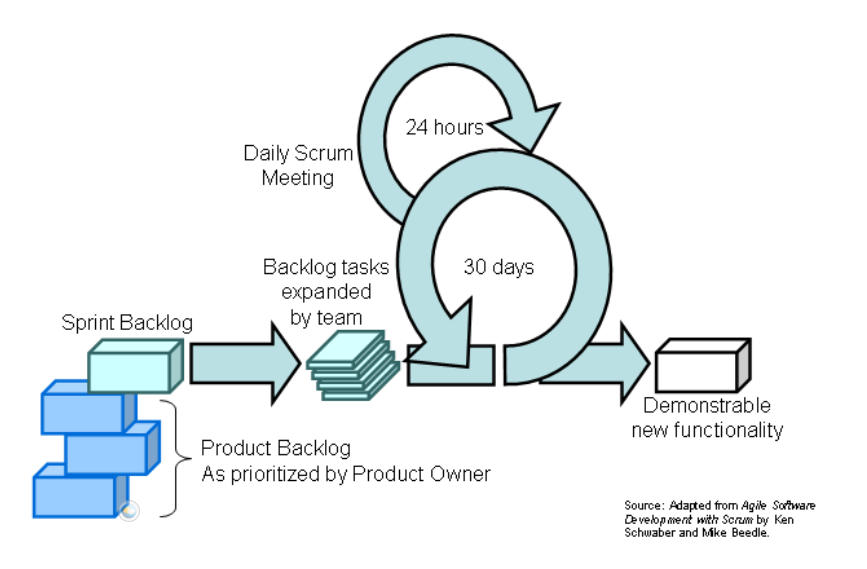
\includegraphics[width=.8\textwidth]{img/tp1_parte2/scrum}
  \caption{Modelo de Trabajo Scrum}
  \label{scrum}
\end{figure}

El producto resultado de un Sprint es el incremento. El incremento tiene como característica que todas las tereas está completamente terminadas y operativas, es decir, en condiciones de ser  entregadas  al cliente. Se detallarán estos resultados en cada uno de los sprint.

No se considerará como incrementos: prototipos, módulos o subrutinas pendientes de pruebas o de integración. Se hará una excepción el primer sprint en el cual se definirán los detalles generales de las tecnologías a utilizar.

\subsection{Product Backlog}

Como se detalló anteriormente, en el product backlog  se recogerán los requerimientos del sistema\/necesidades de los clientes, sobre estos requerimientos se realizará una estimación de tiempo necesario para concretarlo, se establecerán prioridades entre los user stories y finalmente se indicará un comentario para el mismo siempre que sea pertinente. 
En la siguiente \textbf{Tabla} podemos apreciar el product backlog del proyecto.
Se recuerda que estos requerimientos representan una primera aproximación a los requerimientos definitivos por lo que no puede considerarse que están establecidas todas y cada una de las características que el producto tendrá finalmente. Estos serán actualizados y refinados constantemente con el paso del tiempo.


{\scriptsize
\begin{tablaUSNumerada}
	\hline
        \multicolumn{1}{|c|}{\textbf{ID}} &
        \multicolumn{1}{|c|}{\textbf{Enunciado de la historia}} &
        \textbf{Prioridad} \\
	\hline
    \endhead
    
    \hline
        \label{infoPerfil} &
        Como paciente, quiero  añadir información de mi perfil de salud o mediciones regulares para que el médico cuente con más y mejor información al momento de realizar el diagnóstico. 
        & 10 de 10
        
        \\
    \hline
        \label{evitarPerdidas} &
        Como paciente, quiero  añadir al sistema mis estudios realizados para evitar posibles pérdidas. 
        & 9 de 10
        
        \\
    \hline
        \label{infoSalud} &
        Como paciente quiero cargar mi información personal de salud referido a mediciones (altura, grasa corporal, peso, presión arterial), para que el médico cuente con más y mejor información al momento de realizar el diagnóstico. 
        & 10 de 10
        
        \\
    \hline
        \label{diagnosticarPaciente} &
        Como médico quiero diagnosticar a un paciente, para darle un cierre a una incidencia planteada por la persona. 
        &7 de 10
        
        \\
    \hline
        \label{cargaCentroSalud} &
        Como paciente, quiero que los sistemas de salud existentes puedan cargar sus resultados directamente en mi carpeta de salud para centralizar mi información. 
        & 7 de 10
        
        \\
    \hline
        \label{asociarDispositivo} &
        Como paciente, quiero asociar un dispositivo para agilizar y ampliar la carga de datos. 
        &4 de 10
        
        \\
    \hline
        \label{categorizarEstudios} &
        Como paciente, quiero categorizar mis estudios por rama de medicina, para lograr una mejor organización y navegabilidad en el sistema. 
        &7 de 10
        
        \\
    \hline
        \label{infoPaciente} &
        Como laboratorio, quiero cargar información de un paciente en su cuenta para ahorrarle las molestias de volver. 
        & 7 de 10
        
        \\
    \hline
        \label{guardarInfoLocal} &
        Como paciente, quiero guardar mi información de manera local para tener un respaldo. 
        &8 de 10
        
        \\
    \hline
        \label{agregarGrupoFamiliar} &
        Como paciente, quiero agregar personas a mi grupo familiar para llevar el seguimiento de los mismos. 
        &8 de 10
        
        \\
    \hline
        \label{modificarPermisos} &
        Como paciente, quiero modificar los permisos de visualización de mis datos con respecto a cada uno de los integrantes de grupo familiar para tener un control total sobre mi privacidad. 
        &4 de 10
        
        \\
    \hline
        \label{comunicarResultado} &
        Como paciente quiero que no sea necesario ir al hospital para que un medico me comunique los resultados del análisis. 
        & 5 de 10
        
        \\
    \hline
        \label{registrarConFacebook} &
        Como usuario quiero registrarme con una cuenta de Facebook y/o Google para facilitar la inscripción al sitio y el manejo de credenciales. 
        &4 de 10
        
        \\
    \hline
        \label{infoHijo} &
        Como mujer embarazada quiero llevar la información de mi hijo para transmitírsela cuando nazca. 
        &2 de 10
        
        \\
    \hline
        \label{graficaParaMedico} &
        Como médico quiero ver gráficas que resuman la información de un paciente para poder ver sus cambios a lo largo de la historia y así apoyar la toma de decisiones y el diagnóstico. 
        &6 de 10
        
        \\
    \hline
        \label{accesoCualquierLugar} &
        Como paciente, quiero acceder a mis documentos desde cualquier lugar para hacer uso de ellos cuando los necesite. 
        & 5 de 10
        
        \\
    \hline
        \label{graficaParaPaciente} &
        Como paciente quiero ver gráficas que resuman mi información en particular para poder ver mis cambios a lo largo de la historia. 
        & 5 de 10
        
        \\
    \hline
        \label{resumenInfo} &
        Como paciente quiero obtener un resumen de mi información de salud básica para hacer uso de la misma en caso de una emergencia. 
        &8 de 10
        
        \\
    \hline
        \label{mostrarComentario} &
        Como paciente quiero ver en un único lugar los comentarios realizados por los médicos autorizados para una lectura rápida. 
        &8 de 10
        
        \\
    \hline
        \label{verificarPaciente} &
        Como médico quiero verificar que las personas que solicitan mi atención sean pacientes para mantener mi cantidad de consultas en una cantidad controlable. 
        &8 de 10
        
        \\
    \hline 
\end{tablaUSNumerada}
}

\subsection{Plan de pruebas}
A continuación detallaremos como llevaremos adelante el plan de pruebas en cada sprint.
\subsubsection{Criterios de aceptación}
Al estar utilizando  metodología ágil se definirá dentro de cada cada sprint, criterios de aceptación. Estos son patrones definidos al inicio de cada sprint, los cuales deben ser satisfechos para que los user stories que conforman el sprint puedan ser finalizados con éxito. Estos criterios son discutidos con todo el equipo de desarrollo y de calidad para que desde el inicio de cada sprint todo el equipo sepa que es lo que se está llevando a cabo en el desarrollo y por qué. Además de esta manera se asegura la calidad en los requerimientos para que no surjan inconvenientes futuros, como pueden ser criterios sin sentido, o mal interpretados.

\subsubsection{Casos de Prueba}
Sobre estos criterios de aceptación se definirán los Casos de Prueba, con un paso a seguir y un resultado esperado. Estos casos de prueba se comenzarán a definir en el comienzo de cada sprint para poder finalizar dentro de la primer semana, de esta forma pueden ser revisado por todo el equipo y que estén todos de acuerdo en que se aprobará lo q realmente se espera

\subsubsection {Ejecución de Pruebas}
Las pruebas se intentaŕan realizar dentro del mismo sprint en que se desarrollo la story y se dará el feedback correspondiente a los desarrolladores, los errores o bugs encontrados por la parte de calidad se llevaran en una planilla, los cuales serán evaluados al comienzo del sprint siguiente para decidir si se incluyen para ser resueltos dentro de dicho sprint o serán resueltos en el futuro.

En el caso en que no se pueda realizar la ejecución de pruebas en el mismo sprint, se trasladará la story con las tareas pendientes al nuevo sprint.

\textbf{Resultados}

%El resultado de las pruebas del sprint incluye casos de prueba fallados, pasados e incidentes identificados. En este apartado se incluirá el estado de las incidencias identificada tanto de la iteración atual como de iteraciones pasadas
Los bugs tiene cuatro estados posibles
\begin{itemize}
	\item \textbf{Abierto:} El bug fue reportado y todavía no está arreglado
    \item \textbf{Cerrado:} El bug reportado, arreglado por el desarrollador y vuelto a testear para verificar que no sigue sucediendo
    \item \textbf{No es bug:}  Lo que fue reportado como un bug, en realidad es una especificación dentro de un user story, por lo que se marca como oque no es un error.
    \item \textbf{Necesito mas información:} Lo que fue reportado por el tester, el desarrollador no lo termina de comprender por lo que pide mas información para poder arreglarlo.
\end{itemize}
\subsection{Pruebas de integración}
Las pruebas de integración serán realizadas una vez que la cantidad de módulos finalizados sea la suficiente como para poder probar el sistema como un todo. Se utilizará un método incremental ascendente ya que se irán probando los módulos específicos para concluir en el módulo que incluya a todos los anteriores.

\section{Objetivos y alcances definitivos \textit{Epics}}
 Se refinaran los objetivos preliminares propuestos con antelación realizando un análisis mas profundo, estructurando el sistema en EPICS, los cuales permitirán organizar los user stories en funcionalidades genéricas del sistema, realizando la descripción correspondiente y  determinando el alcance que se llevará a cabo en cada uno de ellos.
 
\subsection{Generar perfil de datos personales}

Se le permitirá al usuario poder ver su información personal, nombre, apellido, fecha de nacimiento, permitiéndole la edición correspondiente de los mismos.

Alcance: Se permitirá realizar la creación de un usuario, permitiendo su posterior edición y mostrando sus datos en la pestaña correspondiente al perfil de usuario. Los datos a mostrar serán nombre, apellido, género y fecha de nacimiento.

		\textbf{User Stories relacionados}
        
		\begin{itemize}
			\item US-\ref{infoPerfil} Como paciente quiero cargar mi información personal de perfil referido a nombre apellido, fecha de nacimiento,  para poder sentirme identificado con el sistema.           	
		\end{itemize}


\textbf{Generar perfil de mediciones}
Se le permitirá al usuario que pueda ver su información personal para que pueda tener un seguimiento de sus últimas mediciones con posibilidad de que posteriormente pueda ver su evolución a través de gráficas y tablas.
Para lograr esta funcionalidad se le brindarán los formularios de carga necesarios para permitirle gestionar su información en el momento que lo desee.


Alcance: Se permitirá la carga y modificación de medidas del peso, dimensiones corporales, medición de glucosa, grasa corporal y colesterol.
%Luego añadir aquellas medidas que
Además en futuros sprints se permitirá registrar información que complete el perfil del paciente como alergias,afecciones crónicas, suplementos y medicamentos, artefactos médicos e incidencias que considere importante.
	% Se permitirá obtener un perfil personal para los casos de emergencia que cuente con la siguiente información: afecciones crónicas, suplementos, medicamento y artefactos médicos

		\begin{itemize}
			\item  US-\ref{infoSalud} Como paciente quiero cargar mi información personal de salud referido a mediciones (altura, grasa corporal, peso, presión arterial), para que el médico cuente con más y mejor información al momento de realizar el diagnóstico.
            \item US-\ref{resumenInfo}  Como paciente quiero obtener un resumen de mi información de salud básica para hacer uso de la misma en caso de una emergencia
		\end{itemize}

\subsection{Permitir al usuario añadir los análisis realizados}

    Esta funcionalidad permitirá al usuario cargar sus análisis y categorizarlos según la rama de medicina a la que pertenece. Esta carga se puede realizar de diversas maneras una de ellas será permitirles sacarle una foto al análisis correspondiente subiéndolo en algún formato de imagen predeterminado.  Otra forma será permitirle al usuario que suba el archivo sin importar el formato en el que se encuentre, este método trae como desventaja que no podrá ver el archivo en linea, sino que deberá descargarlo. El último método que le permitiremos utilizar al usuario es que la carga del archivo se realice desde donde se realizo el análisis, para esto hemos de utilizar un API y nos adecuaremos a los correspondientes estándares electrónicos de información.
    En todos los casos se deberá  indicar el nombre, tipo de análisis y a que especialidad corresponde 
    
    Alcance: Se desarrollará el modulo de carga de estudios permitiendo que el usuario pueda cargar todo tipo de archivos. 
    
    Se ofrecerá una API de acceso para la carga y lectura de información por parte de agentes externos a nuestro sistema a través de una interfaz web y de dispositivos móviles permitiéndole al usuario dueño de la información gestionar los correspondientes permisos para esto.
    
    Se permitirá clasificar la documentación a través de ciertas ramas de la medicina definidas por defecto en el sistema permitiendo el uso de ``tags'' personalizados.
    
    	\textbf{User Stories relacionados}
	    \begin{itemize} 
	    	\item US-\ref{evitarPerdidas} Como paciente, quiero  añadir al sistema los estudios realizados para evitar posibles perdidas. 
		    \item US-\ref{cargaCentroSalud}  Como paciente quiero que los sistemas de salud existentes puedan cargar sus resultados directamente en mi carpeta de salud para centralizar mi información
			\item  US-\ref{categorizarEstudios} Como paciente quiero categorizar mis estudios por rama de medicina, para lograr una mejor organización y navegabilidad en el sistema
			\item US-\ref{infoPaciente} Como laboratorio, quiero cargar información de un paciente en su cuenta para ahorrarle las molestias de volver.
    	\end{itemize}
    

\subsection{Permitir acceso único y privado a la información}

Se brindará la seguridad necesaria para que el usuario se sienta seguro al cargar su información y no corra el riesgo de que un usuario no permitido acceda a la misma.
Se permitirá el acceso a los datos solo a los dueños y a quienes estos hayan autorizado.

Alcance:
Se permitirá el acceso a la información a través de una cuenta privada que podrá acceder desde plataformas web o teléfonos móviles registrandose desde una cuenta de Facebook o Google. Además se le ofrecerá al usuario la posibilidad de exportar su información a su base de datos local o de imprimirlo si el lo desea.

        \textbf{User Stories relacionados}
        \begin{itemize}
			\item US-\ref{guardarInfoLocal}  Como paciente, quiero guardar mi información de manera local para tener un respaldo.
			\item US-\ref{guardarInfoLocal}Como usuario quiero registrarme con una cuenta de Facebook y/o Google para facilitar la inscripción al sitio y el manejo de credenciales
			%\item Como paciente quiero elegir que información subir al sistema compartido para que solo cierta información este compartida en la nube
			%\item Como médico quiero visualizar la información de un paciente para apoyar la toma de decisiones y el diagnóstico.
			\item US-\ref{accesoCualquierLugar}  Como paciente, quiero acceder a mis documentos desde cualquier lugar para hacer uso de ellos cuando los necesite.            
		\end{itemize}


\subsection{Permitir a los usuarios generar vistas de su información a lo largo del tiempo, a través de gráficas , tablas y resúmenes}.

	Se generaran tablas y gráficas a partir de los datos cargados, para facilitar el proceso de interpretación y así permitirle al usuario descubrir, prevenir, informar o predecir ciertas características referidas a su salud.

	Esta funcionalidad está especialmente dedicada para los médicos ya que son ellos quienes harán una verdadera interpretación de los resultados, así todo esta funcionalidad también la puede utilizar el paciente.
    
	Para la generación de gráficas, se generarán tablas con los datos recopilados indicando la fecha respectiva de cada uno de ellos.
	Se le dará la posibilidad al usuario de decidir en que tipo de gráfica ver la información, que análisis ver, los rangos de fechas en los que desea verlas, y si desea realizar alguna comparación con otros análisis.

	Posibles gráficas a ofrecer:
	\begin{itemize}
   		\item Gráfico circular
	   \item Gráfico de barras
	   \item Ojiva o gráfica de frecuencia acumulada
	   \item Histograma
	   \item Gráficas de dispersión.
	\end{itemize}
    
	Alcance: Se desarrollará el modulo de visualización de datos que consiste en presentar uno o varios resultados de un período de tiempo, de diferentes maneras, ya sea tanto en formato de tablas como de gráficos para poder observar su evolución. 

        
        
        \textbf{User Stories relacionados}
        \begin{itemize}
			\item US-\ref{graficaParaPaciente}  Como paciente quiero ver gráficas que resuman mi información en particular para poder ver mis cambios a lo largo de la historia.
			\item US-\ref{graficaParaMedico} Como médico quiero ver gráficas que resuman la información de un paciente para poder ver sus cambios a lo largo de la historia y así apoyar la toma de decisiones y el diagnóstico.
		\end{itemize}     
        
        
\subsection{Permitir realizar comentarios, a usuarios autorizados, sobre información compartida.}

    Se le permitirá al usuario seleccionar cualquier información de su cuenta y compartirla, ya sea con usuario específico (doctor o paciente) o de forma pública para cualquier usuario, y de este modo permitir que los otros usuarios realicen un comentario sobre la misma. Esta funcionalidad está especialmente destinada a que los médicos puedan realizar un diagnóstico sobre su paciente sin necesidad de que este tenga que dirigirse hasta el centro de salud.
    
    Alcance: 
    Se realizará una sección de comentarios que permitirá al paciente ver todos los comentarios realizados por el médico en cada una de las especialidades que el seleccione.
    Se permitirá la interacción a través de mensajes con el paciente y comentarios sobre incidencias.
    Se le dará la posibilidad al médico para aceptar o no, a personas como sus pacientes antes de recibir información de los mismos o solicitudes.
    
        \textbf{User Stories relacionados}
        \begin{itemize}
			\item US-\ref{mostrarComentario} Como paciente quiero ver en un único lugar los comentarios realizados por los médicos autorizados para una lectura rápida.
            \item US-\ref{comunicarResultado} Como paciente quiero que no sea necesario ir al hospital para que un medico me comunique los resultados del análisis.
			%\item Como médico quiero comentar estudios de un paciente para tener una forma de comunicación directa con el paciente.
			\item US-\ref{verificarPaciente} Como médico quiero verificar que las personas que solicitan mi atención sean pacientes para mantener mi cantidad de consultas en una cantidad controlable.
			\item US-\ref{diagnosticarPaciente} Como médico quiero diagnosticar a un paciente, para darle un cierre a una incidencia planteada por la persona.
		\end{itemize}
        
        
\subsection{Permitir al dueño de la cuenta asignar permisos CRUD (Create, Read, Update, Delete) a otros usuarios.}

    Se le permitirá al usuario gestionar otros perfiles  relacionados con el, siempre y cuando estos últimos estén de acuerdo con este tipo de gestión.
    El tipo de gestión antes nombrado se refiere a aquellos casos en los que una persona que quiera usar el sistema para almacenar datos y obtener información, no sea capaz por si sola de hacerlo ya sea porque no esté capacitado o porque no tiene acceso a un dispositivo tecnológico que se lo permita..
    Un ejemplo de el caso de una madre con su hijo. La madre desea mantener la información de su hijo, cargando al sistema los análisis, modificando la información del mismo, y solicitando asesoramiento a un especialista.

    Alcance: se permitirá la creación de cuentas asociadas a otras, su gestión de permisos y de acceso a la información.
    %Se permitirá la gestión total de los permisos de acceso a la información propia.
    %se permitirá la creación de cuentas asociadas a otras y su gestión de permisos.
    %Se desarrollará el módulo de creación de cuentas asociadas donde se podrá dejar información compartida para la cuenta del hijo.
    
        \textbf{User Stories relacionados}
        \begin{itemize}
			
			\item US-\ref{agregarGrupoFamiliar} Como paciente quiero agregar personas a mi grupo familiar para llevar el seguimiento de los mismos.
			\item US-\ref{modificarPermisos} Como paciente, quiero modificar los permisos de visualización de mis datos con respecto a  cada uno de los integrantes de grupo familiar para tener un control total sobre mi privacidad.
			\item US-\ref{infoHijo} Como mujer embarazada quiero llevar la información de mi hijo para transmitírsela cuando nazca
		\end{itemize}
        

\subsection{Como paciente, quiero asociar un dispositivo para agilizar y ampliar la carga de datos.}

		\textbf{User Stories relacionados}
		\begin{itemize}
			\item US-\ref{asociarDispositivo} Como paciente, quiero asociar un dispositivo para agilizar y ampliar la carga de datos.
		\end{itemize}
        
        
\section{Sprint 0: Preparación y planificación del proyecto}
El objetivo de este sprint es preparar al proyecto desde una perspectiva tecnológica, metodológica y organizativa, antes de comenzar el desarrollo, para así facilitar la preparación y la puesta en marcha de cada sprint.

Muchas de las actividades que abarca el Sprint 0 ya fueron descriptas en secciones anteriores de este documento, decisiones como que puesto tomará cada integrante del equipo en la metodología ágil, análisis de la situación actual, relevamiento generales, fueron detalladas de forma extensa con anterioridad.

\subsection{Definición de puestos de trabajo}
En este apartado se detallaran que actividades realizará cada integrante al desarrollar el sistema.

\begin{table}[h]
\begin{center}
\resizebox{\textwidth}{!}{
\begin{tabular}{|l|c|c|c|c|}
	\hline                      & Back-end      & Front-end    & DevOps & Tester     \\
	\hline Canizo, Franco       & \checkmark    &              &               & \checkmark \\
	\hline Manganiello, Michael & \checkmark    &              & \checkmark    & \checkmark \\
	\hline Morales, Yanina      &               &  \checkmark  &               & \checkmark \\
	\hline Terreno, Iván        &               & \checkmark   &               & \checkmark \\
	\hline \textbf{Total}       & \textbf{2}    & \textbf{2}   & \textbf{1}    & \textbf{4} \\
\hline
\end{tabular}
}
\caption{Equipo de trabajo}
\label{equipoDeTrabajo}
\end{center}
\end{table}



\begin{itemize}
	\item \textbf{Back-end:} 
    
   El Back-End es el área que se dedica a la parte lógica de un sitio web, es el encargado de que todo funcione como debería, el back-end es la parte de atrás que de alguna manera no es visible para el usuario ya que no se trata de diseño, o elementos gráficos, se trata de programar las funciones que tendrá un sitio. El Back-End es la programación dura y pura, desde la programación de las funciones del sitio hasta bases de datos e incluso mas.


    Los responsables de esta parte del proyecto usarán \textbf{Flask}, éste es un framework minimalista, caracterizado por su simplicidad y flexibilidad, escrito en Python y basado en la especificación WSGI de Werkzeug y el motor de templates Jinja2. Tiene la licencia BSD.
    
    La elección de esta herramienta está fundada
    \item \textbf{Front-end:}
    
     En diseño de software, el front-end, es la parte del software que interactúa con el o los usuarios y, el back-end, es la parte que procesa la entrada desde el front-end. La separación del sistema en front-ends y back-ends es un tipo de abstracción que ayuda a mantener las diferentes partes del sistema separadas. La idea general es que el front-end sea el responsable de recolectar los datos de entrada del usuario, que pueden ser de muchas y variadas formas, y los transforma ajustándolos a las especificaciones que demanda el back-end para poder procesarlos, devolviendo generalmente una respuesta que el front-end recibe y expone al usuario de una forma entendible.
     
    Los responsables de esta parte del proyecto usarán \textbf{AngularJS}, éste es un framework de JavaScript de código abierto, mantenido por Google, que ayuda con la gestión de lo que se conoce como aplicaciones de una sola página. Su objetivo es aumentar las aplicaciones basadas en navegador con capacidad de Modelo Vista Controlador (MVC), en un esfuerzo para hacer que el desarrollo y las pruebas sean más fáciles.
    
    Como Framework de la palicación web usaremos \textbf{Bootstrap 3.2.0+}, el cual contiene plantillas de diseño con tipografía, formularios, botones, cuadros, menús de navegación y otros elementos de diseño basado en HTML y CSS, así como, extensiones de JavaScript opcionales adicionales.
    
    \item \textbf{DevOps:}
    
    DevOps es un acrónimo inglés de development (desarrollo) y operations (operaciones), que se refiere a una metodología de desarrollo de software que se centra en la comunicación, colaboración e integración entre desarrolladores de software y los profesionales de operaciones en las tecnologías de la información (IT). DevOps es una respuesta a la interdependencia del desarrollo de software y las operaciones IT. Su objetivo es ayudar a una organización a producir productos y servicios software rápidamente.
    
    Por el momento se ha asignado un único responsable al cargo, el cuál usará \textbf{Shipable}, este es un una plataforma hosteado en la nube que proporciona integración continua, implementación y pruebas a los repositorios de GitHub y Bitbucket.
    
    \item \textbf{Test:}
    
    En el Front-end se utilizará \textbf{Jasmin} junto con \textbf{Karma}. Jasmin es un framework de testing open source para código JavaScript y Karma es una potente herramienta por consola de comando que permite crear y ejecutar tests unitarios creados por Jasmin. 
    
\end{itemize}


{\scriptsize
\begin{center}
\begin{longtable}{|p{6cm}|c|c|c|c|}
    \hline
        \textbf{Tarea} &
        \textbf{Duración} &
        \textbf{Inicio} &
        \textbf{Fin} &
        \textbf{Responsable}\\
    \hline
        \textbf{Sprint 0} & 48 días & 11/03/15 & 27/04/15 &\\
    \hline
          Investigar aplicaciones similares existentes & 6 días & 11/03/15 & 16/03/15 & Equipo completo\\ \hline
  Documentar justificación del proyecto & 5 días & 17/03/15 & 21/03/15 & Equipo completo \\ \hline
  Investigar y definir lenguajes de programación & 2 días & 22/03/15 & 23/03/15 & Equipo completo \\ \hline
  Investigar y definir herramientas y repositorio de documentación & 2 días & 24/03/15 & 25/03/15 & Equipo completo\\ \hline
  Investigar y definir frameworks & 3 días & 24/03/15 & 26/03/15& Equipo completo \\ \hline
  Investigar y definir herramientas y entornos de desarrollo & 2 días & 27/03/15 & 28/03/15& Equipo completo \\ \hline
  Investigar y definir tipos de bases de datos & 3 días & 29/03/15 & 31/03/15 & Equipo completo\\ \hline
  Investigar y definir herramientas de gestión de configuración & 2 días & 01/04/15 & 02/04/15 & Equipo completo\\ \hline
  Configurar repositorio de gestión de configuración & 3 días & 03/04/15 & 05/04/15& Equipo completo \\ \hline
  Investigar y definir issue tracker & 2 días & 06/04/15 & 07/04/15& Equipo completo \\ \hline
  Configurar issue tracker y mapear información del proyecto & 3 días & 08/04/15 & 10/04/15& Equipo completo \\ \hline
  Capacitarse en las tecnologías de desarrollo definidas & 25 días & 03/04/15 & 27/04/15& Equipo completo \\ \hline
  Definir visión, alcance y objetivos del proyecto & 6 días & 22/03/15 & 27/03/15& Equipo completo \\ \hline
  Definir historias de usuario & 3 días & 28/03/15 & 30/03/15& Equipo completo \\ \hline
  Definir importancia y estimación inicial de las historias de usuario & 5 días & 31/03/15 & 04/04/15& Equipo completo \\ \hline
  Definir Epics & 2 días & 05/04/15 & 06/04/15& Equipo completo \\ \hline
  Definir Sprints & 3 días & 07/04/15 & 09/04/15& Equipo completo \\ \hline
  Estimar capacity del equipo & 2 días & 10/04/15 & 11/04/15& Equipo completo \\ \hline
  Definir y documentar perfiles del equipo, estructura, cantidades y funciones principales & 4 días & 12/04/15 & 15/04/15& Equipo completo \\ \hline
  Documentar conceptos fundamentales de la metodología ágil aplicada & 2 días & 16/04/15 & 17/04/15& Equipo completo \\ \hline
  Documentar medios de comunicación utilizados & 2 días & 18/04/15 & 19/04/15& Equipo completo \\ \hline
  Documentar las herramientas y entornos utilizados & 4 días & 20/04/15 & 23/04/15& Equipo completo \\ \hline
  Instalar entornos de desarrollo & 4 días & 24/04/15 & 27/04/15& Equipo completo \\ \hline
\end{longtable}
\end{center}
}

\subsection{Preparación del entorno de desarrollo de Back-end}
Se utilizó PIP como gestor de paquetes para instalar las librerías de Python necesarios. Se pretende armar un entorno correcto que se describe a continuación.
\begin{itemize}
\item alembic==0.7.6 
\item aniso8601==1.0.0
\item Flask==0.10.1
\item  Flask-Migrate==1.4.0
\item  Flask-RESTful==0.3.2
\item  Flask-Script==2.0.5
\item  Flask-SQLAlchemy==2.0
\item gunicorn==19.3.0
\item  itsdangerous==0.24
\item  Jinja2==2.7.3
\item  Mako==1.0.1
\item  MarkupSafe==0.23
\item  psycopg2==2.6
\item pytz==2015.4
\item six==1.9.0
\item SQLAlchemy==1.0.4
\item Werkzeug==0.10.4
\end{itemize}



\subsection{Preparación del entorno de desarrollo de Front-end}
Para el scaffolding se utilizará Yeoman, esta herramientas es descripta en la página oficial como:
\begin{quote}Un robusto conjunto para el lado del cliente compuesto por herramientas y frameworks que pueden ayudar a los desarrolladores a crear rápidamente bonitas aplicaciones web
\end {quote}


Yeoman es un conjunto de herramientas construidas sobre\textbf{ Node.js} que se integra con Grunt y que lleva a cabo una serie de tareas bajo demanda para agilizar el proceso de inicio del desarrollo, esto bajo  la construcción de un esqueleto bastante completo para el tipo de aplicación web que estés haciendo, este procedimiento también es conocido como scaffolding. Además se encargará de comprimir imágenes o hasta de minificar el CSS.
El escaffolder resultante se muestra en la \textbf{Figura \ref{scaffold}}
Para hacer uso de Yeoman es necesario instalar otros programas a parte de Yeoman en sí mismo.
\begin{itemize}
\item \textbf{Node.js v0.10.x+:} Tecnología del lado del servidor basada en el motor  de JavaScript V8, utiliza un sistema de E/S asíncrono y basado en eventos y callbacks de funciones. Esto supone una mayor velocidad de respuesta. Además es esencial para poder usar Yeoman, Grunt y Bower.
\item \textbf{Npm (which comes bundled with Node) v2.1.0+}
\item \textbf{Git:} Es un software de control de versiones diseñado por Linus Torvalds, pensando en la eficiencia y la confiabilidad del mantenimiento de versiones de aplicaciones cuando éstas tienen un gran número de archivos de código fuente.
\item \textbf{Bower:} Es un gestor de paquetes, librerías y dependencias desarrollado por Twitter, que permite descargar automáticamente lo que se necesite para el proyecto y coloque los archivos donde se lo indique. 
\item \textbf{Grunt CLI:} Procesador de tareas, y watchers, que permite automatizar el compilado de los archivos en varios. Permitirá compilar varias salidas al mismo tiempo, en diferentes formatos, según lo que se necesite.
\end{itemize}


Yeoman nos guiará en la instalación tanto de \textbf{Bootstrap 3.2.0+} como de  \textbf{Angular 1.3.0+} con un simple \$ Yo Angular que se puede visualizar en  la \textbf{Figura \ref{yeomanInstall}}

\begin{figure}[h]
  \centering
  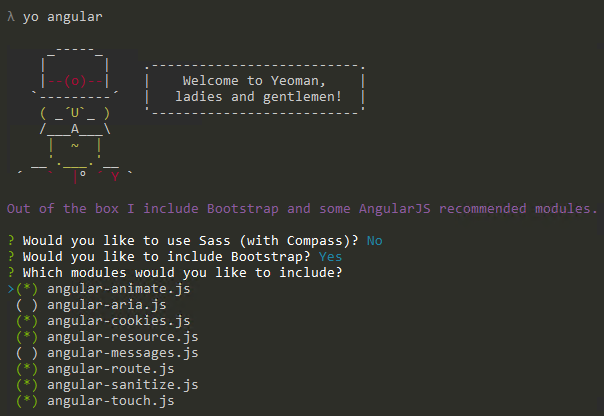
\includegraphics[width=.4\textwidth]{img/tp1_parte2/0-instalacionConYeoman}
  \caption{Confifuración inical de Yeoman}
  \label{yeomanInstall}
\end{figure}

Una vez terminada la configuración de Yeoman, en la carpeta del proyecto tendremos el esqueleto necesario para empezar a trabajar. En la  \textbf{Figura \ref{scaffold}} podemos ver cuales son los directorios principales, siendo estos \textbf{\textit{app}} donde se encuentran las imagenes, los controladores y las vistas y el directorio \textbf{\textit{test}} donde se encuentran los test respectivos para cada uno de los controladores.

\begin{figure}[h]
  \centering
  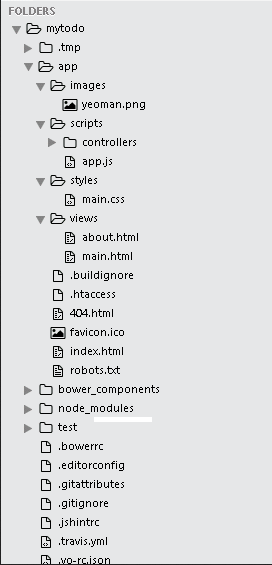
\includegraphics[width=.4\textwidth]{img/tp1_parte2/0-scaffold}
  \caption{scaffold de la aplicación inicial}
  \label{scaffold}
\end{figure}

\subsection{Diagrama de clases tentativo}
{\correccionTexto
En la \textbf{Figura \ref{2-modelo_datos_general}} se presenta el diagrama de clases tentativo, dicho diagrama  será utilizado como base a lo largo de los futuros sprint a desarrollar y posee un alcance limitado el cual se irá modificando a medida que se profundice en los temas.

Para realizar este diagrama se utilizaron los user stories definidos con anterioridad y el relevamiento que se ha realizado hasta el momento, pero como se dijo anterirormente, muchos de los temas serán profundizados en cada Sprint.
}

\begin{correccionSidewaysFigure}
  \centering
  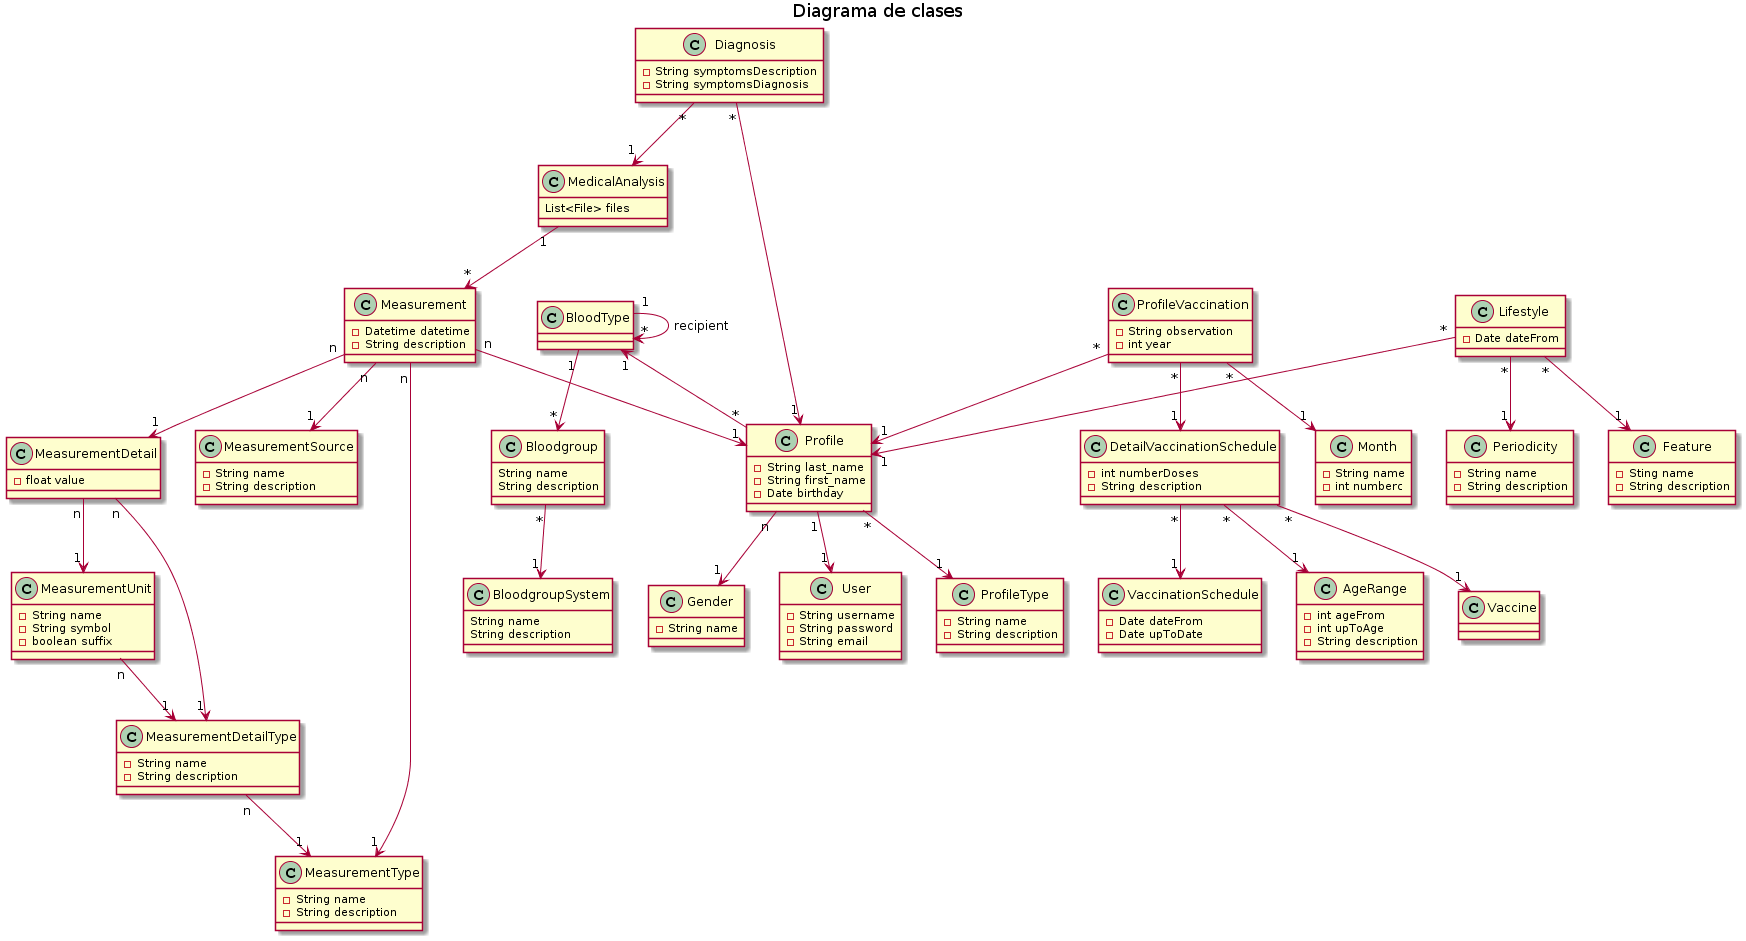
\includegraphics[width=0.9 \textwidth]{img/tp1_parte2/0-DiagramaClasesGeneral}
  \caption{Modelo de datos General}
  \label{2-modelo_datos_general}
\end{correccionSidewaysFigure}


\clearpage % Lo hice para que la imagen del scaffold no me quede tan abajo
\section{ Sprint 1: Generar perfil de datos personales}
\subsection{Planificación}
Inicio: Martes 28 de abril del 2015.

Fin: Martes 19 de mayo del 2015.

\subsection{Descripción:}
En este sprint se realizará la sección del perfíl del usuario, para lo cual se deberá definir en el backend, las clases Profile y Gender, así como los recursos para acceder a ellas a través de la API. Además se realizara la documentación correspondiente para su consumo.
Por parte del frontend se debe desarrollar los recursos de acceso a la API, las vista HTML y cada uno de sus controladores: Una para mostrar el perfíl y otra de edición del mismo.

Para lograr brindarle esta funcionalidad se desarrollarán los formularios de carga y edición para permitirle gestionar su información en el momento que lo desee.

\subsection{User Stories relacionados}
{\scriptsize
\begin{table}[h]
	\begin{tabular}{|l|p{10cm}|c|}
	\hline
        \multicolumn{1}{|c|}{\textbf{ID}} &
        \multicolumn{1}{|c|}{\textbf{Enunciado de la historia}} &
        \textbf{Prioridad} \\     
    \hline
        US-\ref{infoPerfil} &
        Como paciente quiero cargar mi información personal nombre, apellido, fecha de nacimiento y más para armar mi perfil e identificarme así en el sistema.& Alta
        \\
    \hline 
	 \end{tabular}
\end{table}
}




\subsection{ Modelo de datos.}

El Diagrama que propio de este sprint se puede ver en la \textbf{Figura \ref{modeloEspecifico}}, allí se indican exactamente las clases que se usarán en este sprint y que serán detalladas con detenimiento en el presente documento. Se recuerda que se ha realizado un Diagrama de clases tentativo que se puede ver en la \textbf{Figura \ref{2-modelo_datos_general}}, dicho diagrama  será utilizado como base para este sprint y posee un alcance limitado el cual se irá modificando a medida que se profundice en los temas.



\begin{figure}[h]
  \centering
  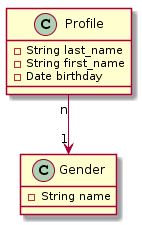
\includegraphics[width=.2\textwidth]{img/tp1_parte2/1-modelo_dato_especifico}
  \caption{Modelo de datos Específico}
  \label{modeloEspecifico}
\end{figure}
\clearpage

\subsection{Descripción de las Clases}

    \subsubsection{ Clase Profile}
    Dicha clase hace referencia a los datos que caracterizan al perfil del usuario.

    \textbf{Descripción de los atributos}
    \begin{itemize}
            \item \textbf{id:}Identificador único del perfil(tipo int)
			\item\textbf{ last\_name 	:}	Apellido de la persona(tipo string).
			\item \textbf{ first\_name: } 	Nombre de la persona (tipo string).
			\item \textbf{birthday 	:}	Fecha de nacimiento de la persona, en formato ISO 8601 (tipo datetime).
			\item \textbf{gender\_id:} 	Identificador único del género asociado 	(tipo int).
    \end{itemize} 
	\textbf{Dirección del recurso:}
    \begin{lstlisting}[language=json,firstnumber=1]
    <BASE URL>/profiles/{:id}
    \end{lstlisting}

    \textbf{Json generado por la API}    
    \begin{lstlisting}[language=json,firstnumber=1]
    {
    "resource": 
    {
    "id": 1,
    "gender": 
    {
    "id": 1,
    "name": "Masculino",
    "description": null
    },
    "birthday": "1990-10-26",
    "last_name": "Terreno",
    "first_name": "Milton"
    }
    }
    \end{lstlisting}

\subsubsection{Clase Gender} 
    \textbf{Descripción de los atributos}
	\begin{itemize}
            \item \textbf{name :}	Nombre del género (tipo string).
            \item \textbf{description 	:}	Descripción del género (tipo string).
    \end{itemize} 
    
    \textbf{Dirección del recurso:}
    \begin{lstlisting}[language=json,firstnumber=1]
    <BASE URL>/genders
    \end{lstlisting}

    \textbf{Json generado por la API}    
        \begin{lstlisting}[language=json,firstnumber=1]
{
    "resource": 
[
{
    "id": 1,
    "name": "Masculino",
    "description": null
},
        {
            "id": 2,
            "name": "Femenino",
            "description": null
        }
    ]
}
        \end{lstlisting}

\subsection{Modelo Funcional}
Se describirán las funciones usando como marco de apoyo el sprint Backlog, además se armará el diagrama de casos de uso del presente Sprint \textbf{[Figura \ref{1-caso_de_uso}]} que irá creciendo  medida se vaya avanzando en el proyecto.
    \begin{figure}[h]
        \centering
        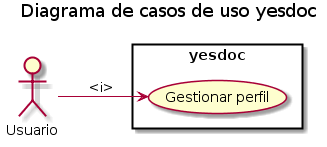
\includegraphics[width=0.5\textwidth]{img/tp1_parte2/1-caso_de_uso}
        \caption{formulario de edición de perfil}
		\label{1-caso_de_uso}
    \end{figure}
	{\scriptsize
	\begin{center} %sidewaystable
	\centering
	%\begin{adjustbox}{max width=\textheight}
    \resizebox{\textwidth}{!}{
	\begin{tabular}{|l|l|l|l|}
	    \hline
	        \textbf{Area a cargo} &
	        \textbf{Responsable} &        
	        \textbf{Tarea} &
	        \textbf{US} \\
	    \hline
	    Front-end & Yanina Morales&  Generación de plantilla principal, con logo, botonera y colores  & US-\ref{resumenInfo} \\ \hline
	    Front-end& Ivan Terreno & Generación de controladores para consumir Json de la Api  & US-\ref{resumenInfo} \& US-\ref{infoSalud} \\ \hline
        Front-end& Ivan Terreno & Capacitación sobre las ventajas de usar resource frente a http & US-\ref{resumenInfo} \& US-\ref{infoSalud}\\ \hline
        Front-end&Ivan Terreno  & Creación de página de perfil&  US-\ref{resumenInfo}\\ \hline
	
    	Back-end&Michael Manganiello  & Creación de aplicación  &  US-\ref{resumenInfo} \& US-\ref{infoSalud}\\ \hline
    	Back-end&Michael Manganiello  & Exposición de métodos como servicios de API 	& US-\ref{resumenInfo} \& US-\ref{infoSalud}\\ \hline
    	Back-end&Franco Canizo   & Adaptación de salida de métodos a formato Json&US-\ref{resumenInfo} \& US-\ref{infoSalud}\\ \hline
    	Back-end&Franco Canizo  & Creación de base de datos inicial&US-\ref{resumenInfo} \& US-\ref{infoSalud}\\ \hline
	    \end{tabular}
        }
	    %\end{adjustbox}
    	\end{center}
	}
    

   \subsubsection{  Generación de plantilla principal, con logo, botonera y colores  }
    
Se generará una plantilla que se utilizará en todas las distintas secciones de la web del proyecto. Esta plantilla incluye los colores principales de la aplicación, un logo representativo \textbf{Figura \ref{logoYesDoc}} y la funcionalidad que permite indicarle al usuario en que lugar esta situado (coloreo de botonera). 

	\begin{figure}[h]
        \centering
        
\includegraphics[width=0.1\textwidth]{img/tp1_parte2/2-logoYesDoc}
        \caption{Logo de la aplicación}
		\label{logoYesDoc}
    \end{figure}

\subsubsection{ Capacitación sobre las ventajas de usar resource frente a http}

Se tuvo que realizar un análisis profundo sobre las ventajas que ofrece resource frente a http en el manejo de recursos brindados por la api, se decidió usar Resource porque proporciona una abstracción a un nivel por encima de \$http, es decir \$resource se vale internamente del objeto \$http y ya implementa CRUD como funciones básicas para persistencia. Al usar resource puede extenderse la base, el ejemplo más usado es modifficar el método update para que se ejecute la actualización por PUT. También trabaja internamente \$q (promises en angular), por tanto podemos usar promises siempre que hagamos una operación contra servidor.

\subsubsection{ Generación de controladores para consumir Json de la Api}
Se generará el código necesario que permita obtener y hacer uso de los Json que genera la API, para esto es necesario crear un resource por cada controlador. En dicho resource se  hará uso de la API  a partir de la especificación de la respuesta brindada y los parámetros requeridos por la misma.

 
\subsubsection{Creación de página de perfil}
En esta tarea  se generará la pantalla del perfil del usuario,\textbf{Figura \ref{perfil}} donde se mostrarán sus datos personales como son:
      \begin{itemize}
	      \item Nombre
          \item Apellido
          \item Fecha de nacimiento
          \item Género
      \end{itemize}
      Para poder presentar los datos del perfil al usuario será necesario  acceder al recurso \texttt{/profiles/\{:d\}} de la API a través de un método 		\textbf{GET}
      
	\textbf{Especificaciones del recursos \texttt{/profiles}}
    
        \begin{lstlisting}[language=json,firstnumber=1]
ProfileFields {
	first_name (string),
	last_name (string),
	id (integer),
	gender (GenderFields, optional),
	birthday (date-time, optional)
}
GenderFields {
	description (string, optional),
	id (integer),
	name (string)
} 
        \end{lstlisting}

	\textbf{Especificaciones del recursos \texttt{/genders}}
        \begin{lstlisting}[language=json,firstnumber=1]
GenderFields {
	description (string, optional),
	id (integer),
	name (string)
} 
        \end{lstlisting}

Además se dará la posibilidad,al usuario, de acceder a la edición de su perfil desde la página de perfil. 


    \begin{figure}[h]
        \centering
        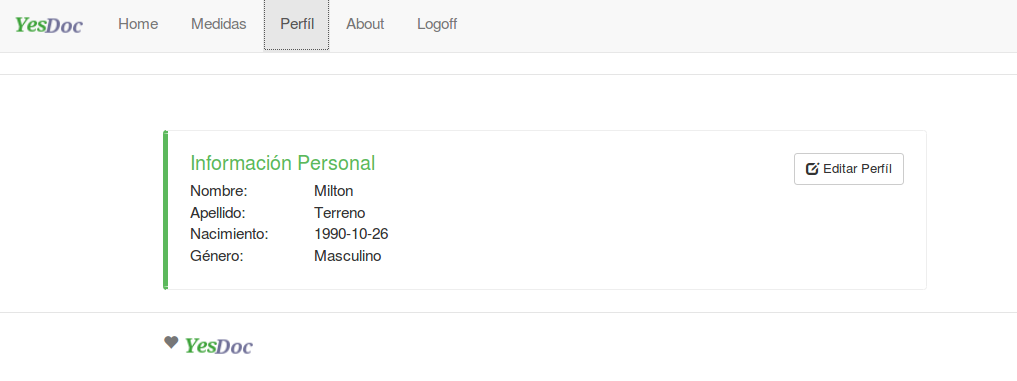
\includegraphics[width=1\textwidth]{img/tp1_parte2/1-perfil}
        \caption{Pantalla de perfil de usuario}
		\label{perfil}
    \end{figure}

\subsubsection{Creación de página de formulario de creación de perfil}      
Se generará el formulario necesario para que el usuario pueda cargar los datos personales antes nombrados. Se presentará una pantalla provisoria de inicio \textbf{Figura \ref{logeo}}  donde se le dará lo opción de logearse o de generar un nuevo perfil.
La opción de \textbf{Nuevo Perfil}, conducirá al usuario al formulario \textbf{Figura \ref{crear_perfil}} donde se realizarán las cargas respectivas de datos
      Para poder crear un nuevo perfil al usuario será necesario  acceder al recurso \texttt{/profiles/\{:d\}} de la API a través de un método \textbf{POST}
    \begin{figure}[h]
        \centering
        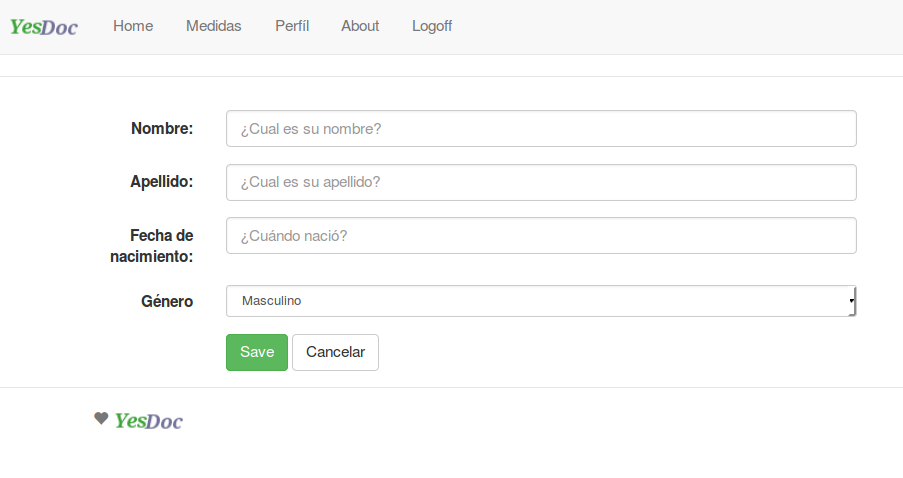
\includegraphics[width=1\textwidth]{img/tp1_parte2/1-crear_perfil}
        \caption{Formulario de creación de perfil}
		\label{crear_perfil}
    \end{figure}
    \begin{figure}[h]
        \centering
        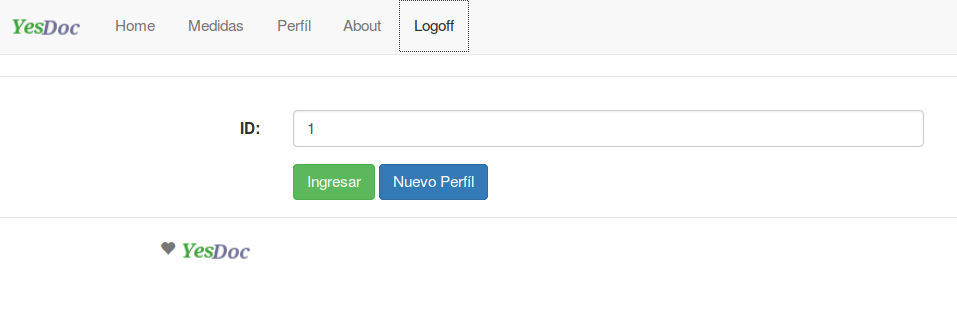
\includegraphics[width=1\textwidth]{img/tp1_parte2/1-logeo}
        \caption{Pantalla de logeo de usuario}
		\label{logeo}
    \end{figure}

\subsubsection{Creación de página de formulario de edición de perfil}      
\begin{figure}[h]
        \centering
        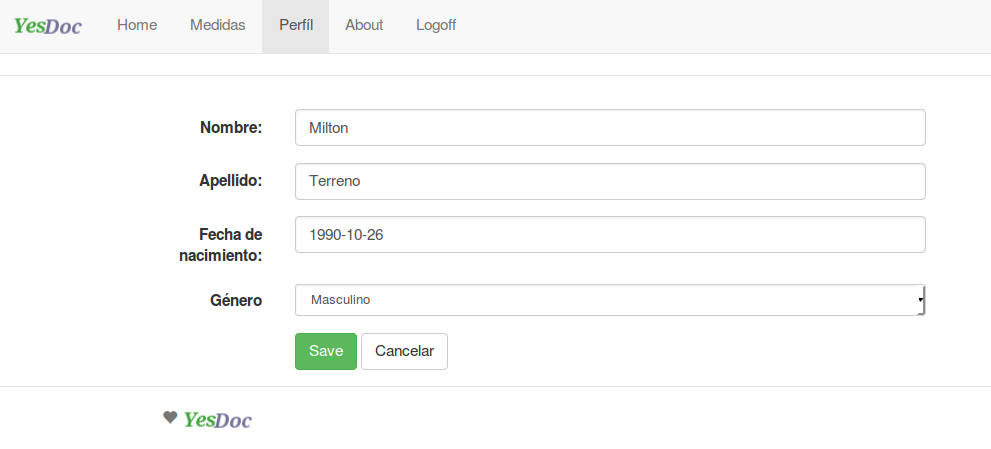
\includegraphics[width=1\textwidth]{img/tp1_parte2/1-editar_perfil}
        \caption{formulario de edición de perfil}
		\label{editar_perfil}
\end{figure}
Se generará el formulario necesario para que el usuario pueda modificar los datos personales antes nombrados. 
En la pantalla de perfil de usaurio \textbf{Figura \ref{perfil}} se le ofrecerá al usaurio la opción de \textbf{Editar Perfil} que lo redireccionará al formulario correspondiente a la edición del perfil, en los campos de dicho formulario se presentarán los datos del perfil, de este modo el usuario solo modificará el campo correspondiente
      Para poder guardar los nuevos datos del perfil al usuario será necesario  acceder al recurso \texttt{/profiles/\{:id\}} de la API a través de un método \textbf{PUT}

    
    
\subsection {Salidas del Sistema - Incrementos}

Luego de finalizado este user story se obtendrá como salida el logo correspondiente a la aplicación que se muestra en la \textbf{Figura \ref{logoYesDoc}}, y 4 pantallas que se detallarán a continuación:
\begin{enumerate}
	\item \textbf{Logeo de usuario:} \textbf{[Figura \ref{logeo}]} Desde esta pantalla el usuario podrá logearse  o crear un perfil nuevo
	\item \textbf{Creación de perfil:}\textbf{[Figura \ref{crear_perfil}]} Se le permitirá cargar aquellos datos que lo identifique nombre, apellido, fecha de nacimiento y género.
    \item \textbf{Presentación de la información personal:} \textbf{[Figura \ref{perfil}]} Aquí se mostrarán los datos personales del usuario (nombre, apellido, fecha de nacimiento y género.), brindándole la posibilidad de edición de los mismos.
    \item \textbf{Edición del perfil:}\textbf{[Figura \ref{editar_perfil}]} En esta pantalla se mostrará el formulario para realizar la edición correspondiente del perfil, los campos estarán precargados con los valores del perfil del usuario, para que este los modifique según disponga.
\end{enumerate}



\clearpage	
\subsection{Planificación de pruebas}
\subsubsection{Criterios de aceptación}


\begin{center}
\begin{longtable}{|p{0.5cm}|p{4cm}|p{4cm}|p{5cm}|}
\hline \rowcolor[gray]{0.9}
	\multicolumn{4}{||c|}{\textbf{Criterio de aceptación}} \\
    \hline  \rowcolor[gray]{0.9}
        \textbf{Id} &
        \textbf{Contexto} &
        \textbf{Evento}&
        \textbf{Resultado} \\
    \hline
        1&En caso de que el usuario exista & y este quiera ingresar al sistema & El sistema le mostrara sus datos personales\\ \hline
        2 &       Si el usuario no existe & y quiere logearse & El sistema no le permitirá ingresar\\ \hline
        3 &       Si el usuario existe y no está logeado & y quiere ingresar a ver su perfil& El sistema no le permitirá ingresar y lo mantendrá en la pantalla de logeo\\ \hline
        4 &       Si el usuario existe & y quiere editar su perfil & El sistema le permitirá modificar cualquiera de sus datos personales\\ \hline
  \end{longtable}
\end{center}

{\correccionTexto
\subsubsection{Pruebas  de  unidad - Casos de Prueba}


	{\scriptsize
    \begin{table} [h]
    \centering
	\begin{tabular}{||l|p{10cm}||}
    	\rowcolor[gray]{0.9}
	    \hline 
        \hline 
       
		\textbf{Caso de prueba} & \textbf{Consultar perfil de usuario existente} \\  \hline
	    \textbf{Descripción del escenario}& Nombre: Marita; Apellido Martinez; fecha de Nacimiento:2015-06-01; género: femenino\\ \hline
	    \textbf{Criterio de aceptación}&  \textbf{En caso de que el usuario exista y este quiera ingresar al sistema. El sistema le mostrara sus datos personales}\\ \hline
        \textbf{Datos de entrada}&  Id:3\\ \hline
        \textbf{Condiciones de  prueba}& Se necesita que esté previamente cargado el usuario "Marita Martinez". \\ \hline \hline
	\end{tabular}
        \caption{Caso de prueba para criterio de aceptación 1}
    \end{table}
	}
 
    	{\scriptsize
        \begin{table}[h]
        \centering
	\begin{longtable}{|p{4cm}|p{6cm}|p{5cm}|}
	    \hline  \hline \rowcolor[gray]{0.9} 
        \multicolumn{3}{||l|}{\textbf{Procedimiento de Prueba - ``Consultar perfil de usuario existente''}} \\
        \hline \rowcolor[gray]{0.9}
	    \textbf{Actor} & \textbf{Sistema}&\textbf{Resultado Esperado} \\  \hline
	   El usuario ingresa en el campo logeo el id:3 & & \\ \hline
        &El Sistema realiza una consulta a la API a partir del id:3 solicitando los datos de la instancia perfil específica&   \\ \hline
        &&Se muestra el  perfil de usuario con sus datos: Nombre: Marita; Apellido Martinez; fecha de Nacimiento:2015-06-01; género: femenino  \\ \hline
	    \end{longtable}
        \caption{Procedimiento de prueba para criterio de aceptación 1}
        \end{table}
	}
    
    {\scriptsize
	\begin{table}[h]
	\centering
	\begin{tabular}{|l|p{10cm}|}
	    \hline 
	    \textbf{Salida obtenida}&Se obtuvieron los datos que se detallaron previamente en ``Resultado esperado''\\ \hline
	    \textbf{Resultado}& \textbf{Correcto}\\ \hline
        \textbf{¿Que fue mal?}& Nada\\ \hline      
        \textbf{Evidencia}&  \\ \hline
        \textbf{Seguimiento}& No es necesario ya que el caso de prueba no causó fallos \\ \hline
        \textbf{Estado}& \textbf{Terminado}\\ \hline        
        \textbf{¿Que se puede mejorar?}& En una futura iteración se podría añadir el grupo sanguíneo y añadir un cartel de bienvenida al sistema \\ \hline              
	    \end{tabular}
        \caption{Resultado esperado para el criterio de aceptación 1}
    	\end{table}
	}
    

    %%%%%%%%   
    
\clearpage    
    
    {\scriptsize
	\begin{table}[h]
	\centering
	\begin{tabular}{||l|p{10cm}||}
    	\rowcolor[gray]{0.9}
	    \hline 
        \hline 
	    \textbf{Caso de prueba} & \textbf{Consultar perfil de usuario No existente} \\  \hline
	    \textbf{Descripción del escenario}&\\ \hline
	    \textbf{Criterio de aceptación}&\textbf{Si el usuario no existe y quiere logearse. El sistema no le permitirá ingresar}\\ \hline
        \textbf{Datos de entrada}&  Id:64\\ \hline
        \textbf{Condiciones de  prueba}& No existe un usuario con id=64 \\ \hline \hline
	    \end{tabular}
        \caption{Caso de prueba para criterio de aceptación 2}
    	\end{table}
	}
    
    {\scriptsize
        \begin{table}[h]
        \centering
	\begin{longtable}{|p{4cm}|p{6cm}|p{5cm}|}
	    \hline  \hline \rowcolor[gray]{0.9} 
        \multicolumn{3}{||l|}{\textbf{Procedimiento de Prueba - ``Consultar perfil de usuario NO existente''}} \\
        \hline \rowcolor[gray]{0.9}
	    \textbf{Actor} & \textbf{Sistema}&\textbf{Resultado Esperado} \\  \hline
	   El usuario ingresa a logearse con el id:64 & & \\ \hline
        & El Sistema realiza una consulta a la API a partir del id:64 solicitando los datos de la instancia perfil específica &   \\ \hline
        &El Sistema detecta que no existe un perfil con id:64&  Se mantiene al usuario en la vista de logueo\\ \hline
	    \end{longtable}
        \caption{Procedimiento de prueba para criterio de aceptación 2}
        
    	\end{table}
    }
    
    {\scriptsize
	\begin{table}[h]
	\centering
	\begin{longtable}{|l|p{10cm}|}
	    \hline 
	    \textbf{Salida obtenida}&El sistema permitió el ingreso a la interfaz de perfil, mostrando los datos vacíos\\ \hline
	    \textbf{Resultado}& \textbf{Fallido} \\ \hline
        \textbf{¿Que fue mal?}& El sistema no le debería haber permitido al usuario ingresar\\ \hline      
        \textbf{Evidencia}& Imagen \ref{prueba2} \\ \hline
        \textbf{Seguimiento}&  {\correccionTexto En la Imagen \ref{correccionprueba2} se pueden ver las modificaciones que tuvieron que hacerse en el código del archivo login.js del controlller para poder resolver el error descubierto, las líneas en rojo son las que se encontraban en un comienzo, las cuales producían error, y tuvieron que ser reemplazadas por las lineas marcadas en verde para que las pruebas pasen. También se puede ver en las figura \ref{Codigoinicialprueba2} como se encontraba el codigo inicialmente.}\\ \hline
        \textbf{Estado}& \textbf{Terminado \& Corregido}\\ \hline        
        \textbf{¿Que se puede mejorar?}& Se corrigieron los errores pero en otra iteración se podría añadir carteles de advertencia, esto se verá en los sprint relacionados a la seguridad\\ \hline              
     
	    \end{longtable}
        \caption{Resultado esperado para el criterio de aceptación 2}
    	\end{table}
	}
    
\begin{figure}[h]
  \centering
  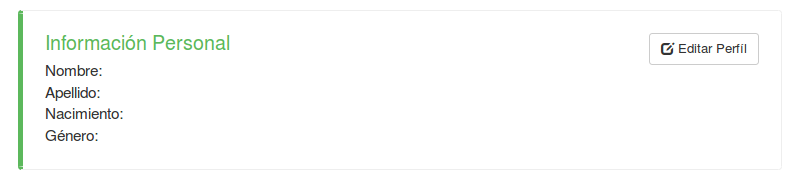
\includegraphics[width=.8\textwidth]{img/tp1_parte2/1-prueba_2}
  \caption{error en la pruebas 2}
  \label{prueba2}
\end{figure}

\begin{figure}[h]
  \centering
  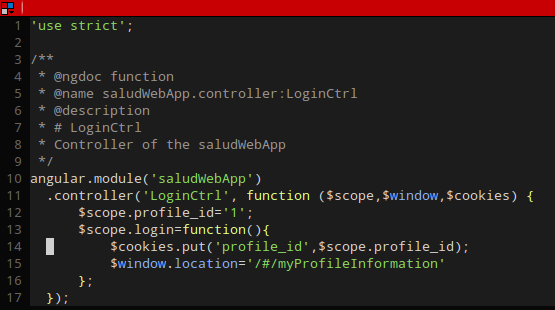
\includegraphics[width=.8\textwidth]{img/tp1_parte2/1-codigo_prueba_2}
  \caption{Codigo utilizado inicialmenete para el logeo}
  \label{Codigoinicialprueba2}
\end{figure}


\begin{correccionFigure}[h]
  \centering
  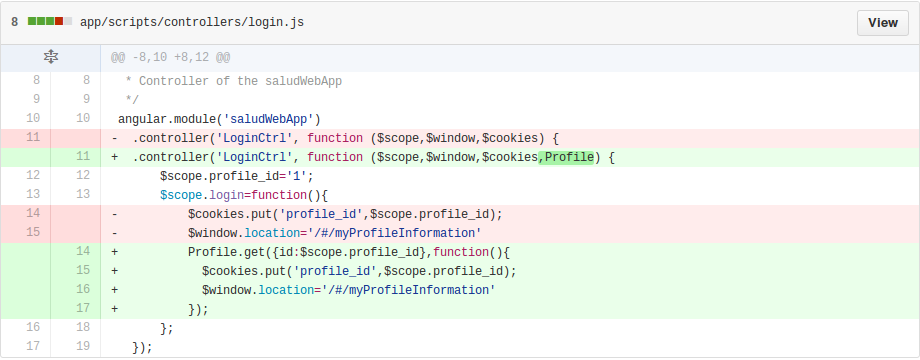
\includegraphics[width=.8\textwidth]{img/tp1_parte2/1-correccion_prueba_2}
  \caption{Correcciones de los error detectados en la pruebas 2}
  \label{correccionprueba2}
\end{correccionFigure}

\clearpage
    %%%%%%%%%%%%%%%%%%%%%%

{\scriptsize
	\begin{table}[h]
	\centering
	\begin{tabular}{||l|p{10cm}||}
    	\rowcolor[gray]{0.9}
	    \hline 
        \hline 
	    \textbf{Caso de prueba} & \textbf{Ingresar al sistema sin logearse} \\  \hline
	    \textbf{Descripción del escenario}& no son necesarios\\ \hline
	    \textbf{Criterio de aceptación}&\textbf{Si el usuario existe y no está logeado y quiere ingresar a ver su perfil, el sistema no le permitirá ingresar y lo mantendrá en la pantalla de logeo}\\ \hline
        \textbf{Datos de entrada}&  ninguno\\ \hline
        \textbf{Condiciones de  prueba}& el usuario no se logea \\ \hline \hline
	    \end{tabular}
        \caption{Caso de prueba para criterio de aceptación 3}
    	\end{table}
	}
    
    {\scriptsize
	\begin{table}[h]
    \centering
	\begin{longtable}{|p{5cm}|p{5cm}|p{4cm}|}
	    \hline \hline \rowcolor[gray]{0.9}
        \multicolumn{3}{||l|}{\textbf{Procedimiento de Prueba - ``Ingresar al sistema sin logearse''}} \\
        \hline 
        \rowcolor[gray]{0.9}
	    \textbf{Actor} & \textbf{Sistema}& \textbf{Resultado Esperado} \\  \hline
	   El usuario selecciona la pestaña de ``perfil'' para ingresar a ver su perfil (sin antes haberse logeado) & & \\ \hline
        & El sistema valida que exista una cookie con las sesión creada&   \\ \hline
        &El Sistema no encuentra una cookie existente y no hace nada&  Se mantiene al usuario en la vista de logueo\\ \hline
	    \end{longtable}
        \caption{Procedimiento de prueba para criterio de aceptación 3}
    	\end{table}
    }
    
    {\scriptsize
	\begin{table}[h]
	\centering
	\begin{longtable}{|l|p{10cm}|}
	    \hline 
	    \textbf{Salida obtenida}&El sistema mantuvo al usuario no logeado en la ventana de logeo, garantizando que no ingrese al sistema\\ \hline
	    \textbf{Resultado}& \textbf{Correcto}\\ \hline
        \textbf{¿Que fue mal?}& Todo salio como se esperaba\\ \hline      
        \textbf{Evidencia}& para esta prueba no es necesaria \\ \hline
        \textbf{Seguimiento}& No es necesario ya que el caso de prueba no causó
fallos \\ \hline
        \textbf{Estado}& \textbf{Terminado}\\ \hline        
        \textbf{¿Que se puede mejorar?}& {\correccionTexto En otra iteración se podría añadir carteles de advertencia, esto se verá en los sprint relacionados a la seguridad }\\ \hline              
	    \end{longtable}
        \caption{Resultado esperado para el criterio de aceptación 3}
    	\end{table}
	}
    

\clearpage
    %%%%%%%%%%%%%%%%%%%%%%%%%%%%

    {\scriptsize
	\begin{table}[h]
	\centering
	\begin{tabular}{||l|p{10cm}||}
    	\rowcolor[gray]{0.9}
	    \hline 
        \hline 
	    \textbf{Caso de prueba} & \textbf{Editar perfil} \\  \hline
	    \textbf{Descripción del escenario}&Nombre: Marita; Apellido Martinez; fecha de Nacimiento:2015-06-01; género: femenino; id:3\\ \hline
	    \textbf{Criterio de aceptación}& \textbf{Si el usuario existe y quiere editar su perfil, el sistema le permitirá modificar cualquiera de sus datos personales}\\ \hline
        \textbf{Datos de entrada }& datos modificados nombre: Marita Emilce\\ \hline
        \textbf{Condiciones de  prueba}&  usuario con id:3 logeado \\ \hline \hline
	    \end{tabular}
        \caption{Caso de prueba para criterio de aceptación 4}
    	\end{table}
	}
    
    {\scriptsize
	\begin{table}[h]
    {\correccionTexto
    \centering
	\begin{longtable}{|p{5cm}|p{5cm}|p{4cm}|}
	    \hline \hline \rowcolor[gray]{0.9}
        \multicolumn{3}{||l|}{\textbf{Procedimiento de Prueba - ``Editar perfil''}} \\
        \hline 
        \rowcolor[gray]{0.9}
	    \textbf{Actor} & \textbf{Sistema}& \textbf{Resultado Esperado} \\  \hline
	   El usuario presiona sobre el botón``editar perfil'' & & \\ \hline
        & El Sistema realiza una consulta a la API a partir del id:3 para traer los datos del perfil y precargar el formulario &   \\ \hline
        & &  Se muestra un formulario con los datos del usuario para que sean modificados\\ \hline
        El usuario modifica su nombre y añade un segundo nombre Emilce&& \\ \hline
        &El sistema carga los nuevos datos a la API a través del método PUT&\\ \hline
        &El sistema redirecciona al usuario a la vista de perfil de usuario&Se muestra el perfil con sus datos y el nuevo nombre ingresado\\ \hline
	    \end{longtable}
        \caption{Procedimiento de prueba para criterio de aceptación 4}
        }
    	\end{table}
    }
    
    {\scriptsize
	\begin{table}[h]
	\centering
	\begin{tabular}{|l|p{10cm}|}
	    \hline 
	    \textbf{Salida obtenida}& El formulario con los datos se mostraron correctamente\\ \hline
	    \textbf{Resultado}& \textbf{Correcto}\\ \hline
        \textbf{¿Que fue mal?}& nada\\ \hline      
        \textbf{Evidencia}& {\correccionTexto En la Imagen \ref{prueba4} se puede ver el formulario con los datos precargados y en el Json \ref{JsonProfile} que contiene los nuevos datos los cuales accedemos a partir de la url \begin{lstlisting} 
https://yesdoc-api.herokuapp.com/profiles/3 \end{lstlisting} }\\ \hline
        \textbf{Seguimiento}& No es necesario ya que el caso de prueba no causó
fallos
\\ \hline
        \textbf{Estado}& \textbf{Terminado}\\ \hline        
        \textbf{¿Que se puede mejorar?}& \\ \hline              
	    \end{tabular}
        \caption{Resultado esperado para el criterio de aceptación 4}
    	\end{table}
	}
\clearpage

\begin{figure}[h]
  \centering
  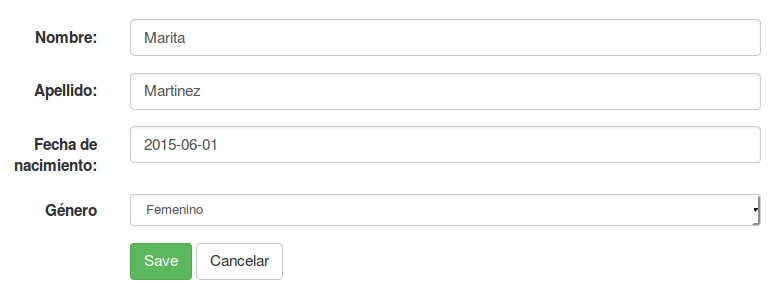
\includegraphics[width=.8\textwidth]{img/tp1_parte2/1-prueba_4}
  \caption{Prueba 4}
  \label{prueba4}
\end{figure}

\begin{lstlisting}[language=json,firstnumber=1,  breaklines=true, caption= Json del perfil id:3 modificado, label=JsonProfile]
{
 "resource": {
    "gender":{
            "description": null,
            "id": 2,
            "name": "Femenino"
        },
        "first_name": "Marita Emilce",
        "last_name": "Martinez",
        "id": 3,
        "birthday": "2015-06-01"
    }
}
\end{lstlisting}
}
\clearpage
    %%%%%
    
    


    
    %%%%
    \clearpage
\subsubsection{Pruebas  de  integración entre módulos del Sistema}
Estas pruebas se realizarán más adelante, en futuros sprints.
\subsubsection{ Pruebas de carga}
En este sprint no se realizarán este tipo de pruebas.
\subsubsection{ Pruebas de seguridad por niveles de usuarios}
En este sprint no se realizarán este tipo de pruebas, ya que la seguridad será un tema a tratar más adelante.

\subsection{Pruebas ejecutadas}
Aqui se realizará una conclusión general de lo que se descubrió en las pruebas.
	\begin{itemize}
		\item \textbf{¿Que fue bien?}
        	\begin{itemize}
				\item Los datos de usuario se mostraron correctamente, además al cargar  los datos no se tuvo inconveniente alguno.
			\end{itemize}
   		\item \textbf{¿Que se mejoró?}
        	\begin{itemize}
				\item \textbf{Cerrado}  Se detecto que cuando un usuario inexistente iniciaba sesión, podía ingresar al módulo de perfil, en este módulo no se mostraban los datos, ya que no existía  el usuario, pero no era correcto que esto sucediera.
                \item \textbf{Cerrado} Se encontraron problemas  con los nav's, los cuales sólo se marcaban como seleccionados cuando se presionaban y esto no nos servía para los casos en los que había que redireccionar. Se solucionó utilizando Angular Strap.
                
			\end{itemize}
   		\item \textbf{¿Qué se puede mejorar?}
        	\begin{itemize}
				\item \textbf{Abierto} Al finalizar el Sprint se vio necesario implementar un item que indique el grupo sanguíneo de la persona.
                \item \textbf{Abierto} Se podría arreglar la forma de seleccionar las fechas en el caso de la "fecha de nacimiento".
                \item \textbf{Abierto} Se deberá añadir, en los sprint relacionados a seguridad, los carteles de advertencia correspondientes.
                \item \textbf{Abierto} En próximas iteraciones deberá añadirse el grupo sanguíneo de la persona
                \item \textbf{Abierto} En próximas iteraciones deberá añadirse un cartel de bienvenida del usuario al sistema.
			\end{itemize}
    \end{itemize}


